\documentclass[letterpaper, 12pt]{article}
\usepackage[top=2cm,bottom=1cm,left=0.75in,right=0.75in,headheight=17pt, % as per the warning by fancyhdr
includehead,includefoot,
heightrounded, % to avoid spurious underfull messages
]{geometry}
\addtolength{\topmargin}{-.25in}
\usepackage{fancyhdr}
\pagestyle{fancy}
\usepackage{graphicx}
\usepackage{lastpage}
\usepackage{gensymb}

\begin{document}
\fancyhead[l]{	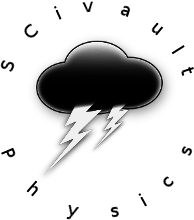
\includegraphics[height=1.2cm]{../Logo/sp.png} Name:}
\fancyhead[r]{REFERENCE MATERIAL}
\cfoot{\thepage\ of \pageref{LastPage}}
	


\begin{center}Things to Memorize: Circuits
\end{center}

\subsection*{Basics of Circuits}
\begin{itemize}
	\item For Electricity to flow, a circuit must make a complete path between the two sides of the source. 
	\item \textbf{Voltage} is the energy per charge.
	\item \textbf{Current} is the amount of charge that passes a point in one second. 
	\item \textbf{Resistance} is the hindrance to the flow of charge.
\end{itemize}
\subsection*{Circuit Components}
\begin{center}
	\begin{tabular}{|c | p{1in} | p{3.5in}  |}
		\hline
		Battery & \vspace{0.5in} &  \textit{Source} - Stores energy for a circuit chemically. \\ \hline
		Resistor &\vspace{0.5in}   &  Dissipates electrical energy as heat; resists the flow of current.    \\ \hline
		Light Bulb & \vspace{0.5in}  & Similar to a resistor, but resistance changes with temperature. \\ \hline
		Light Emitting Diode (LED) &  \vspace{0.5in}  & Turns electrical enegy into light; only lets current flow one way.  Must be used in series with a resistor or will be destroyed.  \\ \hline
		Capacitor &  \vspace{0.5in} & Stores energy in an electrical field.   \\ \hline
		Inductor & \vspace{0.5in} & Stores energy in a magnetic field. \\ \hline
		Ammeter & \vspace{0.5in} & Measures current \\ \hline 
		Voltmeter & \vspace{0.5in} & Measures Voltage \\ \hline		
	\end{tabular}
\end{center}
	
\subsection*{Resistors}
	

\subsection*{Capacitors}

\subsection*{Types of Circuits}
	\begin{itemize}
		\item \textbf{Series circuits} have only one path for current to flow.
			\begin{itemize}
				\item Resistors in Series \textbf{add}.
				\item Capacitors in Series \textbf{add as reciprocals}.
				\item Current in series is \textbf{the same}.
				\item Voltage in series \textbf{adds up} to the voltage of the source. 
			\end{itemize}
		\item \textbf{Parallel Circuits} have multiple paths for current to flow. 
		\item Some circuits have parts that are in series and other parts that are in parallel.
	\end{itemize}
\subsection*{Meters and Measurements}

\subsection*{Kirchhoff's Laws}


 



\end{document}
